\section{Zielsetzung}
In diesem Versuch soll der Phasenübergang von Wasser von flüssig zu gasförmig untersucht werden.
Dafür soll die Verdampfungswärme des Wassers in Abhängigkeit der Temperatur ermittelt und insbesondere eine Dampfdruckkurve
erstellt werden.

\section{Theorie}
Allgemein kann Wasser die Phasen fest, flüssig und gasförmig annehmen. Diese Phasen lassen sich in einem Zustandsdiagramm (s. Abbildung \ref{fig:theorie1})
darstellen. In dem Zustandsdiagramm ist der Druck $p$ gegen die Temperatur $T$ aufgetragen und mit Hilfe dreier Kurven lassen sich Bereiche abgrenzen, die 
die Phasen definieren. In den durch die Kurven abgegrenzten Arealen hat das System die zwei Freiheitsgrade $p$ und $T$.\\
Sobald sich der Punkt $(T{,}\,p)$ einer der Kurven nähert erreicht man Zustände in denen zwei Phasen koexistieren. Dies ist für die Punkte TP. und K.P. der Fall, die
auch den Anfangs- und Endpunkt der Dampfdruckkurve charakterisieren.\\
\label{sec:Theorie}
\begin{figure}
    \centering
    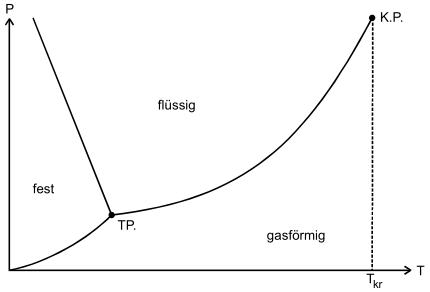
\includegraphics{Theorie1.png}
    \caption{qualitatives Zustandsdiagramm des Wassers [\cite{sample}}, S. 176]
    \label{fig:theorie1}
\end{figure}
\\
Auf der Dampfdruckkurve hat das System nur noch einen Freiheitsgrad, da $p$ und $T$ nicht mehr beliebig wählbar sind. Diese Kurve wird durch die Verdampfungswärme $L$
charakterisiert. Dabei ist $L$ eine stoffabhängige, temperaturabhängige Größe und verschwindet im kritischen Punkt (K.P.) fast gänzlich. Dennoch ist $L$ in einem Temperaturbereich 
in dem die Messung stattfinden soll fast konstant.\\
\\
Die molare Verdampfungswärme $L$ gibt an wie viel Energie in Joule benötigt werden, um ein Mol eines Stoffs verdampfen zu lassen. Um die mathematische Herleitung zu verstehen, stelle
man sich ein evakuiertes Gefäß vor, das zum Teil mit Wassermolekülen gefüllt ist. Da die Wassermoleküle der Maxwellschen Geschwindigkeitsverteilung gehorchen, gibt es Moleküle
mit maximaler kinetischer Energie, die die Flüssigkeitsoberfläche verlassen. Dabei leisten sie Arbeit gegen die molekularen Kräfte. Dieser Prozess
heißt Verdampfung und die dafür benötigte Energie wird entweder von außen hinzugefügt oder dem Wasser in Form von Wärme entnommen. Bei dem umgekehrten Prozess der Kondensation wird
diese Energie wieder frei.\\
Die Gasmoleküle erzeugen nun einen Druck, da sie gegen die Wände des Gefäßes stoßen. Außerdem können die Gasmoleküle, die auch sich nach der Maxwellschen
Geschwindigkeitsverteilung verhalten, wenn sie auf das Wasser treffen wieder eingefangen werden, so dass sich auf Dauer ein Gleichgewichtszustand einstellt. 
Wenn das Gleichgewicht erreicht ist, gilt der Verdammpfungsvorgang als abgeschlossen. Dann stellt sich ein Druck ein, der als Sättigungsdruck bezeichnet wird.
Da bei höherer Temperatur die Geschwindigkeitsverteilung zu höheren Geschwindigkeiten verschoben wird, steigt bei der Sättigungsdruck an. Dabei ist zu beachten, dass der Druck nicht
vom Volumen abhängt, so dass die ideale Gasgleichung
\begin{equation}
    \label{eqn:allgGasgl}
    pV = RT
\end{equation}
nicht verwendet werden kann.
\\
\\
Formel zum Zitieren schonmal
\begin{align}
    \label{eqn:druck}
    p = exp(ln(p_0))\cdot exp(-\frac{L}{RT}) \\
    ln(p) = -\frac{L}{RT} + ln(p_0)
\end{align}

\cite{sample}
